\subsection{Toy Gridworld Domain}

In this section, we run Q-learning and Sarsa with linear function approximation in the two gridworld domain shown in Figure \ref{fig:gridworld1} and Figure \ref{fig:gridworld2}. The results of the experiments are shown in Figure \ref{fig:1} and Figure \ref{fig:2} for the domain 1 and 2 respectively. All the algorithms were averaged over $50$ independent trials and each trial consisted of $6000$ episodes.

\textbf{Experiment 1 (Domain 1):} In this experiment we use linear function approximation for both Q-Learning and Sarsa to handle this partially observed environment. From Figure \ref{fig:1} we see that Sarsa performs better than Q-Learning in this Domain and stabilizes before Q-Learning.

\textbf{Experiment 2 (Domain 2):} In this experiment again we use linear function approximation for both Q-Learning and Sarsa to handle this partially observed environment. From Figure \ref{fig:2} we see that Sarsa performs worse than Q-Learning in this Domain. Infact both the algorithms does not stabilize in this experiment. This results from the fact the the entry to the state $S_t = G$ is restricted and both the algorithms spend considerable amount of time in fruitless exploration.


\begin{figure}[!th]
    \begin{center}
    \begin{tabular}{cc}
    \setlength{\tabcolsep}{0.1pt}
    \subfigure[2.75\textwidth][Expt-$1$: $10\times 10$ Gridworld (Domain 1)]
    %with $r_{i_{{i}\neq {*}}}=0.07$ and $r^{*}=0.1$
    {
    		\pgfplotsset{
		tick label style={font=\large},
		label style={font=\large},
		legend style={font=\large},
		ylabel style={yshift=12pt},
		%legend style={legendshift=32pt},
		}
        \begin{tikzpicture}[scale=0.8]
      	\begin{axis}[
		xlabel={Episodes},
		ylabel={Discounted Return},
		grid=major,
        %clip mode=individual,grid,grid style={gray!30},
        clip=true,
        %clip mode=individual,grid,grid style={gray!30},
  		legend style={at={(0.5,1.4)},anchor=north, legend columns=3} ]
      	% UCB
		\addplot table{results/NewExpt/Expt1/comp_subsampled_QlearningA.txt};
		\addplot table{results/NewExpt/Expt1/comp_subsampled_SarsaA.txt};
		\addplot table{results/NewExpt/Expt1/comp_subsampled_QlearningL.txt};
		\addplot table{results/NewExpt/Expt1/comp_subsampled_SarsaL.txt};
      	\legend{Q-Learning, Sarsa, Q($\lambda$), Sarsa($\lambda$)}   
      	\end{axis}
      	\end{tikzpicture}
  		\label{fig:1}
    }
    &
    \subfigure[2.75\textwidth][Expt-$2$: $10\times 10$ Gridworld (Domain 2)] 
    %with $r_{i_{{i}\neq {*}}}=0.07$ and $r^{*}=0.1$
    {
    		\pgfplotsset{
		tick label style={font=\large},
		label style={font=\large},
		legend style={font=\large},
		ylabel style={yshift=12pt},
		%legend style={legendshift=32pt},
		}
        \begin{tikzpicture}[scale=0.8]
      	\begin{axis}[
		xlabel={Episodes},
		ylabel={Discounted Return},
		grid=major,
        %clip mode=individual,grid,grid style={gray!30},
        clip=true,
        %clip mode=individual,grid,grid style={gray!30},
  		legend style={at={(0.5,1.4)},anchor=north, legend columns=3} ]
      	% UCB
		\addplot table{results/NewExpt/Expt2/comp_subsampled_QlearningA.txt};
		\addplot table{results/NewExpt/Expt2/comp_subsampled_SarsaA.txt};
		\addplot table{results/NewExpt/Expt2/comp_subsampled_QlearningL.txt};
		\addplot table{results/NewExpt/Expt2/comp_subsampled_SarsaL.txt};
      	\legend{Q-Learning, Sarsa, Q($\lambda$), Sarsa($\lambda$)}   	
      	\end{axis}
      	\end{tikzpicture}
  		\label{fig:2}
    }
    \end{tabular}
    \end{center}
    \caption{A comparison of the performance of various algorithms. }
    \label{fig:algoExpt}
    \vspace*{-1em}
\end{figure}

\subsection{Classic Domain}

The mountain car was first described in Andrew Moore's Thesis \citep{Efficient memory-based learning for robot control} and was latter properly defined in \citet{DBLP:journals/ml/SinghS96}. The task consist of driving a car resting in a valley up the mountain. The main challenge of this task is that the car by itself cannot drive up the mountain and it has to swing back and forth to gather the sufficient momentum to reach the top of the mountain (see Figure \ref{fig:3}). Nonetheless, this simple environment consist of several challenges that afflicts the medical domain. It's a continuous state space problem, hence function approximation has to be used which makes it a partially observed MDP. Moreover, the car can only accumulate a positive reward of $+50$ when it reaches the top or suffers a negative reward of $-1$ the time while it swings back and forth.  So this models the long horizon problem. The action space is discrete in this toy domain. 

In Figure \ref{fig:4} we show how Q($\lambda$) and Sarsa($\lambda$) along with Fourier basis can be used to solve this problem.

\begin{figure}[!th]
    \begin{center}
    \begin{tabular}{cc}
    \setlength{\tabcolsep}{0.1pt}
    \subfigure[2.75\textwidth][Domain-$3$: Mountain Car]
    %with $r_{i_{{i}\neq {*}}}=0.07$ and $r^{*}=0.1$
    {
    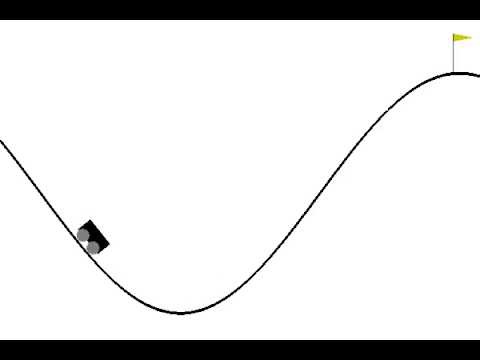
\includegraphics[scale=0.35]{img/mountain_car.jpeg}
    \label{fig:3}
    }
    \setlength{\tabcolsep}{0.1pt}
    \subfigure[2.75\textwidth][Expt-$3$: Mountain Car]
    %with $r_{i_{{i}\neq {*}}}=0.07$ and $r^{*}=0.1$
    {
    		\pgfplotsset{
		tick label style={font=\large},
		label style={font=\large},
		legend style={font=\large},
		ylabel style={yshift=12pt},
		%legend style={legendshift=32pt},
		}
        \begin{tikzpicture}[scale=0.8]
      	\begin{axis}[
		xlabel={Episodes},
		ylabel={Discounted Return},
		grid=major,
        %clip mode=individual,grid,grid style={gray!30},
        clip=true,
        %clip mode=individual,grid,grid style={gray!30},
  		legend style={at={(0.5,1.4)},anchor=north, legend columns=3} ]
      	% UCB
		\addplot table{results/NewExpt/Expt3/comp_subsampled_Qlearning.txt};
		\addplot table{results/NewExpt/Expt3/comp_subsampled_Sarsa.txt};
		\addplot table{results/NewExpt/Expt3/comp_subsampled_Qlearning1.txt};
		\addplot table{results/NewExpt/Expt3/comp_subsampled_Sarsa1.txt};
      	\legend{Q-Learning, Sarsa, Q($\lambda$), Sarsa($\lambda$)}   
      	\end{axis}
      	\end{tikzpicture}
  		\label{fig:4}
    }
    \end{tabular}
    \end{center}
    \caption{A comparison of the performance of various algorithms. }
    \label{fig:algoExpt1}
    \vspace*{-1em}
\end{figure}
